\documentclass[12pt]{article}


\usepackage[dvips,letterpaper,margin=0.75in,bottom=0.75in]{geometry}
\usepackage{cite}
\usepackage{slashed}
\usepackage{graphicx}
\usepackage{amsmath}

\usepackage[american,fulldiode,oldvoltagedirection]{circuitikz}
\tikzset{component/.style={draw,thick,circle,fill=white,minimum size =0.75cm,inner sep=0pt}}

\begin{document}
\ctikzset{bipoles/thickness=1}
\ctikzset{bipoles/length=0.6cm}

\title{Introduction to the Arduino} 

\maketitle

\section{Introduction}

\begin{figure}[htbp]
\begin{center}
 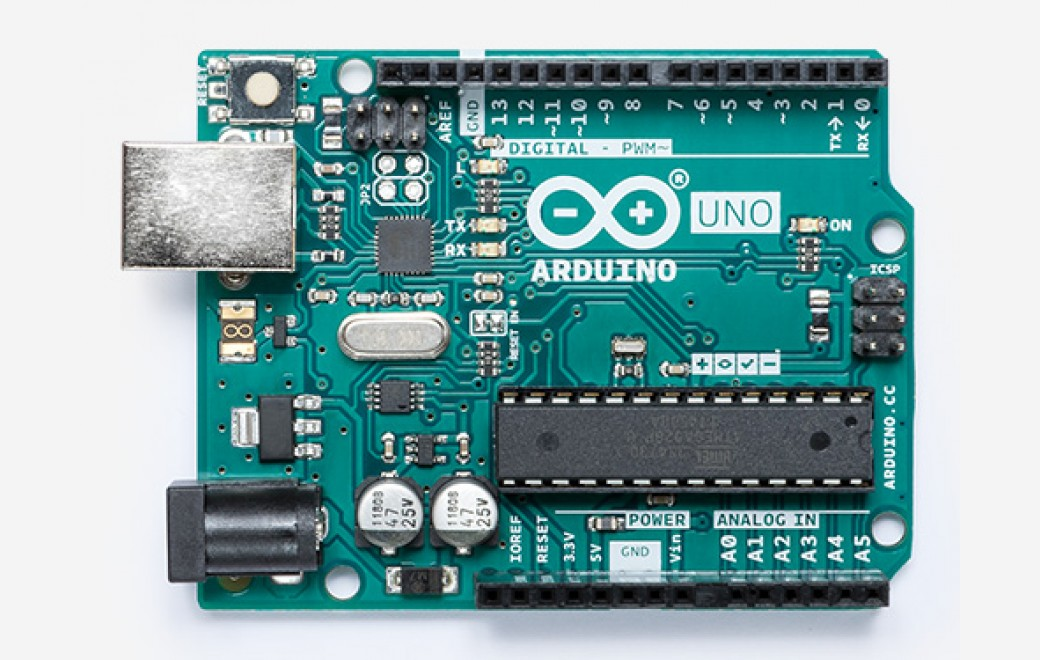
\includegraphics[width=0.55\textwidth]{figs/uno.jpg};
\caption{\label{fig:uno} The Arduino Uno microprocessor.}
\end{center}
\end{figure}

In this lab, we will learn to use the Arduino microprocessor, which we
will be using for the hands on portion of this course.  The model we
will use is the Arduino Uno.  You should keep a text log file, which
you will submit on the course website once you have completed this
assignment.

\section{Getting Started with the Arduino}

\noindent
{\bf Step 1:} Your Arduino should have arrived pre-installed with a
custom shield.  Remove the shield for these initial tests as
demonstrated at the end of the hardware checkout video, being careful
not to damage the pins.

\vspace{0.5 cm}    
\noindent
{\bf Step 2:} The main Arduino website, which includes lots of
supporting documentation, is located at {\tt http://arduino.cc}.
Acquaint yourself with this site.

\vspace{0.5 cm}
\noindent
{\bf Step 3:} You should have already installed the Arduino software.
Follow the instructions for using the ``Arduino Desktop IDE" located here:  
{\tt https://www.arduino.cc/en/Guide/ArduinoUno}.

\vspace{0.5 cm}
\noindent
{\bf Step 4:} Compile and upload the LED blink example.  Take a close
look at the program, which is enough to understand the most important features of an Arduino sketch.

\vspace{0.5 cm}
Your Arduino microprocessor runs a single program which you can
create, modify, compile, and upload in the Arduino integrated
development environment IDE.  For this lab, the sketches will have
only two function of interest.  The {\tt setup()} function is called
once when the program first starts (such as upon reset, or opening a
serial connection).  This is where you do things that only need to be
done once, such as setting the LED pin to an output in the Blink
example.  The {\tt loop()} function is run in an endless loop: the
program calls {\tt loop()} immediately after finishing setup, and the
program calls {\tt loop()} again as soon as it finishes.  The
execution of loop can be momentarily interrupted by special interrupt
signals, but we won't be using interrupts directly in this lab.  In
the Blink example, the {\tt loop()} function turns on the LED, pauses
for one second, turns off the LED, and then pauses for a second.  The
LED blinks repeadedly because it reenters the loop function
immediately on exiting.  Each blink you observe is one call to
{\tt loop()}

You'll be starting from example sketches throughout these labs that
already define the functions {\tt setup()} and {\tt loop()} but you
will need to keep their roles in mind when decided where to put your
modfications.

\vspace{0.5 cm}
\noindent
{\bf Step 5:} Adjust the pattern of the LED blink example to a slower rate.  Record your modification in your logbook.

\vspace{0.5 cm}
\noindent
{\bf Step 6:}  The Arduino tutorials and built-in-examples are often excellent starting points for you own projects, browse the tutorials here:\\
https://www.arduino.cc/en/Tutorial/HomePage

\section{The 116C custom proto-board}

The features included in your custom proto-board are shown in
Fig.~\ref{fig:features}.  This lab will not use the $RC$ filter, but
will make use of the LED, push-button, and potentiometer. 

\begin{figure}[htbp]
\begin{center}
\begin{tabular}{c@{\hskip 0.2cm}c@{\hskip 0.2cm}c@{\hskip 0.2cm}c@{\hskip 0.2cm}c}
\begin{circuitikz}[line width=1pt]
  \draw (0,0) node[left]{pin $5$} to[short,o-] ++(1.0,0.0) to[resistor,l=$R$] ++(0,-4.0)
  to[short,-o] ++(-1.0,0.0) node[left]{pin $8$};
\end{circuitikz} &
\begin{circuitikz}[line width=1pt]
  \draw (0,0) node[left]{pin $A5$} to[short,o-] ++(1.0,0.0) to[C,l=$C$] ++(0,-4.0) node[ground,yscale=2.0]{};
\end{circuitikz} &
\begin{circuitikz}[line width=1pt]
  \draw (0,0) node[left]{pin $11$} to[short,o-] ++(1.0,0.0) to[resistor,l=$R$] ++(0,-2.0) coordinate(X)
  to[led, bipoles/length=1.0cm] ++(0,-2.0) node[ground,yscale=2.0]{};
\end{circuitikz} &
\begin{circuitikz}[line width=1pt]
  \draw (0,0) node[left]{$5~\rm V$} to[short,o-] ++(1.0,0.0) to[resistor,l=$R$] ++(0,-2.0) coordinate(X)
  to[push button,bipoles/length=1.5cm, l=S] ++(0,-2.0) node[ground,yscale=2.0]{};
  \draw (X) to[short,-o] ++(-1.0,0.0) node[left]{pin $2$};
\end{circuitikz} &
\begin{circuitikz}[line width=1pt]
  \draw (0,0) node[left]{pin $A2$} to[short,o-] ++(1.0,0.0)
  to[american potentiometer,n=mypot,l_=R] ++(0,4) to[short,-o] ++(-1.0,0.0) node[left]{pin $A0$}  
  (mypot.wiper) to[short,-o] ++(-0.8,0) node[left]{pin $A1$};
\end{circuitikz} \\

(a) & (b) & (c) & (d) & (e)\\
\end{tabular}
\caption{The features already implemented on the custom proto-board.
  The (a) $220~\rm \Omega$ resistor and (b) capacitor are used for RC
  filtering in the digital scope lab, the (c) current limited LED is
  controlled by pin 11, the (d) user switch $S$ pulls pin 2 to ground
  when pressed, and a (e) $10~\rm k\Omega$ potentiometer has the wiper
  connected to analog pin $A1$.}
\label{fig:features}
\end{center}
\end{figure}

\vspace{0.5 cm}
\noindent
{\bf Step 1:} While the proto-board is off the Arduino, take some time
to see how the various features are implemented.  The components are
on top, but some connections are made on the bottom with wired
connections.  Work through the diagrams and make sure you see how each
component is connected to the Arduino pins.

\vspace{0.5 cm}
\noindent
{\bf Step 2:} Carefully reinstall the custom proto-board shield which
you removed in the previous section, as demonstrated at the end of the
hardware checkout video, being careful not to damage the pins.

\vspace{0.5 cm}
\noindent
{\bf Step 3:} Modify the LED blink example to make use of the red LED
on the proto-board, instead of the built in LED.  Record your
modifications in your logbook.

\vspace{0.5 cm}
\noindent
{\bf Step 4:} The DigitalInputPullup example works as provided because
it expects a user switch connected to pin 2 exactly as on your
protoboard.  This sketch will turn on the onboard LED underneath the
protoshield while you press the switch.  Modify it to blink the red
LED on the proto-board instead.  Record your modifications in your logbook.

\vspace{0.5 cm}
Analog output on the Arduino UNO is accomplished by Pulse Width
Modulation (PWM).  A PWM output is a digital signal (either 0 or VCC)
but with a variable duty cycle. The output for value 0 is always off,
and the output for value 255 is always on, but the output for value
123 will be on one half of each cycle and off for one half of each
cycle.  The {\bf average} voltage is therefore a programmable analog
value between 0 and VCC.  To get a truly analog value, you need some
sort of filtering, such as from an $RC$ filter, appropriate for the
PWM rate, which is configurable but around 1 kHz on the UNO.

Your eye is a high-pass filter, you cannot perceive an LED blinking at
the PWM rate, so we can use PWM to dim an LED.  The LED is always
fully on or fully off, but your eye perceives the faction of time it
is on for each cycle as brightness.

\vspace{0.5 cm}
\noindent
{\bf Step 5:} Modify the LED fade example to make use of the red LED
on the proto-board, instead of the built in LED.  Record your
modifications in your logbook.  

\vspace{0.5 cm}
We'll receive analog inputs from the potentiometer shown in
Fig.~\ref{fig:features}D.  The wiper is connected to pin $A1$ which we
will use as input.  To function as a potiometer, the end of the
variable resistance need to be set to ground and VCC.  Since analog
pins can be used as digital outputs, we'll simply write a digital 1 to
A0 and digital 0 to A2.

\vspace{0.5 cm}
\noindent
{\bf Step 6:} Run the AnalogReadSerial example on your Arduino.  Open
the serial monitor tool making certain that the baud rate is set to
same value used by sketch (Serial.begin()).

\vspace{0.5 cm}
This sketch takes its input from pin A0, so you won't see the values
change as you turn the knob on the potiometer.

\vspace{0.5 cm}
\noindent
{\bf Step 7:} Change the pin used for analogRead to A1 (from A0).  Record your change in your logbook.

\vspace{0.5 cm}
\noindent
{\bf Step 8:} Add the following lines to the Setup function in your sketch, which setup pins A0 and A1 as ground and VCC for the potiometer:
\begin{verbatim}    
  // The potentiometer is installed at A0-A1-A2.
  // Set A0 to VCC and A2 to ground
  pinMode(A0, OUTPUT);
  pinMode(A2, OUTPUT);
  digitalWrite(A0, HIGH);
  digitalWrite(A2, LOW);  
\end{verbatim}

\vspace{0.5 cm}
\noindent
{\bf Step 9:} Now as you adjust the knob, you should see the serial
output range from full scale at 1023 (nominally 5 V) down to 0
(nominally 0 V).  For a graphical view, exit the serial monitor and
use the serial plotter.  You should see the value move around on the
plot as you turn the knob.  {\tt Rename your modified sketch and save
  it for later... it's a good starting point for the next section}.
    
\section{Digital Control System}

You now have everything that you need to make a digital control system
for the LED.  Create a sketch that allows you to dim the LED based on
the setting of the potentiometer.  Do this digitally!

One approach is to start from the analogRead serial example, as
modified to work with our potentiometer as described above.  Then,
understand and import the parts of the LED fade example that are
useful for your purposes.

Keep in mind that analog read values are from 0 to 1023 (10 bit
values) while analog write values are from 0 to 244.  So convert the
value you read from the potiometer to a value you can use in a call to
{\tt analogWrite()}, you will have to divide by four.

This is the main design portion of the lab.  Completing the
preliminary steps is enough for ``B''.  Completing this design is
needed for an ``A''.  Once you have it working, you should upload your
single *.ino file with your completed design along with your text file
log.

\section{Design Improvements}

For fun and extra credit, you can develop any or all of these
alternative designs.  The TA will only provide limited help on these
problems and at lower priority than helping with required portions of
the labs:
\begin{itemize}
\item There is an analog solution for creating the LED dimmer.
  Instead of controlling the LED by using pin 11 as a PWM output, set
  pin 11 as an input which will make it high impedance.  Then, connect
  the output of the potentiometer directly to the pin 11.
\item Make the LED blink briefly and then remain off for a time
  controlled by the setting of the potentiometer.
\item Use the push button to switch between two or more LED modes,
  such as dimming and variable rate blinking.  You'll want to debounce
  the switch using a technique like the example
  DigitalStateChangeDetection.
\item These are just ideas... if there's something else you want to try, give it a go!
\end{itemize}
Don't submit extra credit with your lab.  There will be an extra
assignment where you can submit extra credit, which can be completed
at any time during the quarter.

 
\end{document}
